\documentclass[aps,prl,floatfix,preprintnumbers,twocolumn,groupedaddress,nofootinbib]{revtex4-1}
\usepackage{amsmath,amsthm,amssymb,color,psfrag,url,latexsym,graphicx,epstopdf,slashed,xspace,hyperref,enumitem}
\hyphenpenalty=500
\usepackage{lineno}

\definecolor{darkred}{rgb}{0.6,0.0,0.0}
\definecolor{darkblue}{rgb}{0.0,0.0,0.5}
\definecolor{darkgreen}{rgb}{0.0,0.5,0.0}
\definecolor{brown}{rgb}{0.0,0.0,0.0}
\newcommand{\red}{\color{darkred}}
\newcommand{\blue}{\color{darkblue}}
\newcommand{\green}{\color{darkgreen}}

\newcommand{\rap}{y}
\newcommand{\be}{\begin{equation}}
\newcommand{\ee}{\end{equation}}
\newcommand{\bea}{\begin{eqnarray}}
\newcommand{\eea}{\end{eqnarray}}

\begin{document}
\preprint{MIT-CTP 4952}
\title{Telescoping Jet Substructure}

\author{Yang-Ting Chien$^{a,d}$}
\email{ytchien@mit.edu\\}

\author{Alex Emerman$^{c,d,e}$}
%\email{alex.emerman@gmail.com}

\author{Shih-Chieh Hsu$^b$}
%\email{schsu@uw.edu}

\author{Samuel Meehan$^b$}
%\email{smeehan12@gmail.com}

\author{Zachary Montague$^{a,b}$}
%\email{zacander.mon@gmail.com}

\affiliation{
$^a$ Center for Theoretical Physics, Massachusetts Institute of Technology, Cambridge, MA 02139\\
$^b$ Department of Physics, University of Washington, Seattle, WA 98195\\
$^c$ Department of Physics, Columbia University, New York, NY 10027\\
$^d$ Theoretical Division, T-2, Los Alamos National Laboratory, Los Alamos, NM 87545\\
$^e$ Physics Department, Reed College, Portland, OR 97202
}

\date{\today}
\linenumbers

\begin{abstract}
We introduce a novel jet substructure calculus, called telescoping jet deconstruction, which exploits the variation of observables with respect to a sampling of phase-space boundaries quantified by the variability. We apply this method to identify boosted $W$ boson and top quark jets using telescoping jet grooming and telescoping subjets, demonstrating its ability to disentangle the information coming from the subjet topology and that coming from the subjet substructure. We find excellent performance of the variability measure, in particular its robustness against finite detector resolution. This method provides a new direction in heavy particle tagging and enables a more complete and systematic approach to the decomposition of jet substructure.
\end{abstract}
\maketitle

The Large Hadron Collider (LHC) has begun to regularly probe physics above the electroweak scale, where the momenta of massive Standard Model particles are much larger than their invariant masses, resulting in hadronic decays of jets with prong-like substructures. Many jet substructure variables have been designed~\cite{Abdesselam:2010pt,Altheimer:2012mn,Altheimer:2013yza} and combined using multivariate techniques~\cite{Adams:2015hiv,Larkoski:2017jix,ATLAS-CONF-2017-064,Khachatryan:1955546} to identify such jets and increase the sensitivity to beyond the Standard Model physics. However, the ability to accurately reconstruct the features of such jets is obscured by the presence of additional proton-proton interactions (i.e. pileup) as well as the underlying event of the hard collision, both of which cause for additional radiation to fall within the catchment area of the jet.  Often, this radiation is removed through one of a number of grooming procedures, i.e. pruning~\cite{Ellis:2009su} or trimming~\cite{Krohn:2009th}.  These observables and grooming procedures target certain intuitive features of the radiation properties and often have tuneable parameters.  For example, in the pruning algorithm, the $z_{\rm cut}$ and $D_{\rm cut}$ parameters control the softness and noncollinearity of a discarded particle. Conventionally, one makes a single choice of parameters deemed optimal by some metric.  However, such a choice may neglect the full information the entire observable class contains.

Recently, the Q-jets technique \cite{Ellis:2012sn} introduced non-determinism in jet clustering. The procedure probes each jet multiple times and quantifies differences among pruned jets using the variability in the mass of the resulting ensemble of pruned jets. This concept can be refined by examining the radiation pattern surrounding the dominant energy flow with multiple angular resolutions $\{R_i\}$, one can extract the full information contained in jets at all angular scales, analogous to that investigated in \cite{Chien:2014hla}. In this Letter we apply this technique, called telescoping jet deconstruction to analyze a set of commonly used jet observables and grooming procedures. We demonstrate the feasibility of the method as applied to the identification of hadronically decaying $W$ bosons and top quarks. Analogous to the Q-jets procedure, where the the mass volatility was used as the final observable, the variability of each observable, under the variation of the parameters of the given algorithm, is used as the fundamental observable.

In hadronic boosted two-body resonance decays, such as a $W$ boson, the resonance mass $M$ introduces a two-prong structure in the jet at an angular scale $\Theta\approx 2M/p_T$ between the two prongs, where $p_T$ is the transverse momentum of the heavy particle. On the other hand, QCD jets initiated by isolated quarks and gluons have such distinct scale. However, when examining jets whose mass is near $M\pm\Delta m$, QCD jets are also two-prong-like but with a more distended radiation pattern when $\Delta m\gg\Gamma$ where $\Gamma$ is the natural width of the resonance. Besides this nontrivial {\sl subjet topology}, the strong interaction dictates the formation of subjets with {\sl subjet substructures} and {\sl subjet superstructures} \cite{Gallicchio:2010sw} which are sensitive to the partonic origins of subjets. 

In the case of boosted top quarks, the top mass ($M_t$) and the $W$ mass ($M_W$) are not hierarchically separated \textbf{\color{blue} SAM : What does hierarchically separated mean? It is not common jargon in my mind.}.  Therefore $\Theta_t \approx 2M_t/p_T^t$ and $\Theta_W \approx 2M_W/p_T^W$ can be comparable. This results in the generic three-prong structure in the hadronic top decay $t\rightarrow W+b \rightarrow q_1 + q_2 +b$. However, when examining jets with a mass near $M_t\pm \Delta m$ the selected QCD jets are again two-prong-like and so observables which distinguish three-prong jets from two-prong jets will help discriminate the such jets from true top quark jets.

Given an arbitrary jet observable $\cal O$ with a parameter $a$,
the variation of the observable with respect to the sampling of parameters $\{a_i\}$ within $(a_{\rm min},a_{\rm max})$, or the {\sl variability}, is quantified by the coefficient of variation $v_{\cal O}^a$ defined as the ratio of the standard deviation and the mean of $\{{\cal O}_{a_i}\}$,
\be
    v_{\cal O}^a = \frac{\sigma({\cal O}_{a_i})}{\langle {\cal O}_{a_i}\rangle}\;.
\ee
Variations with respect to multiple varied parameters can be studied using the variability matrix. Much like the first derivative in calculus, the variability $v_{\cal O}^a$ measures the change of the observable $\cal O$ with respect to the change of the phase space boundary set by the parameter $a$. Instead of combining observables with different parameters in a multivariate analysis, the variability can give a trend of the observable variation which itself can be used as a distinguishing feature of signal and background jets.

\begin{figure*}
    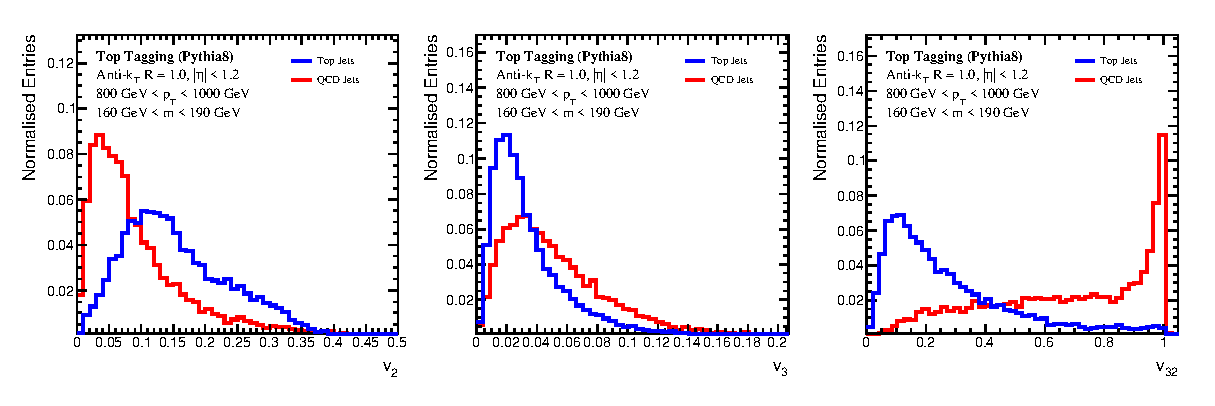
\includegraphics[width=2\columnwidth]{plots/Top_vs_high.eps}
    \caption{The distributions of the variabilities $v_2$ (left panel) and $v_3$ (middle panel), as well as their ratio $v_{32}$ (right panel) for top and QCD jets with $800~{\rm GeV} < p_T < 1~{\rm TeV}$ and $160~{\rm GeV} < m < 190~{\rm GeV}$ using the truth particle information.}
\label{v32}
\end{figure*}

We consider a variety of telescoping deconstruction applications. We focus on the variability of the jet mass with respect to varying the parameters which determine the jet constituents contributing to the jet mass. %observable. In the construction of the variability variables, t
The sampling of the telescoping parameters is uniform within the range $(a_{\rm min},a_{\rm max})$. %\\[-10pt]
\newline
\newline
\noindent \textit{\textbf{Telescoping pruning}}: Using the $k_T$ reclustering algorithm, pruning discards soft and noncollinear particles when %the following condition is satisfied in the merging of particles $i$ and $j$,
merging particles $i$ and $j$ if the combination is both soft and wide-angled,
\bea
    &&\frac{{\rm min}(p_{T_i},p_{T_j})}{|p_{T_i}+p_{T_j}|}<z_{\rm cut}~~~~{\rm (soft)}\nonumber\\
    &&\Delta R_{ij} > D_{\rm cut}\;,~~~~~~~~~~~{\rm (noncollinear)}
\eea
where $p_{T_i}$ are the particle transverse momenta and $\Delta R_{ij}=\sqrt{\Delta y_{ij}^2+\Delta \phi_{ij}^2}$ is the distance between the particles $i$ and $j$ rapidity $y$ and azimuthal angle $\phi$. We fix $z_{\rm cut}=0.1$ and construct $v_{\rm prun}$, the variability of the pruned jet mass with the telescoping parameter $a\in (0.1, 2.0)$ in $D_{\rm cut} = a~ 2m_{\rm jet}/p_{T_{\rm jet}}$. %\\[-10pt]
\newline
\newline
\noindent \textit{\textbf{Telescoping trimming}}: Trimming \cite{Krohn:2009th} reclusters jets into subjets using the $k_T$ algorithm with subjet radius $R_{\rm sub}$. The subjet $i$ is discarded if it is soft, i.e. %the following softness condition is satisfied,
\be
    p_{T_i} < f_{\rm cut}~p_{T_{\rm jet}}\;.~~~{\rm (soft)}
\ee
Here $p_{T_i}$ is the transverse momentum of the $i^{th}$subjet. We construct $v_{\rm trim}$, the variability of the trimmed jet mass with the telescoping parameter $a = f_{\rm cut} \in (0.0, 0.1)$. %\\[-10pt]
\newline
\newline
\noindent \textit{\textbf{Telescoping subjets}}: $N$ subjets are exclusively reconstructed around %to identify the 
dominant energy flows within jets. A similar method using the leading subjets in a reclustered jet was explored in \cite{Cui:2010km}. We choose the subjet axes as the $N$-subjettiness axes \cite{Thaler:2010tr} with $\beta = 1$, and build subjets around them with radius $R_T$ \cite{Stewart:2010tn,Chien:2013kca,Stewart:2015waa,Thaler:2015xaa}. %One can also use the winner-take-all axes. 
Particles are assigned to the nearest axis according to the distance $\Delta R_{ij}$ between the axis $\hat n_i$ and the particle $j$,
\begin{equation}
    {\rm subjet}_{i} = \{p_j~|~\Delta R_{ij}<R_T~{\rm and}~\Delta R_{ij}<\Delta R_{kj}\;,~\forall k\neq i\},
\end{equation}
where $k$ is the index of the other axes $\hat n_k$. The variability $v_N$ of the invariant masses of the sum of $N$ subjets is reconstructed with the telescoping parameter $a = R_{T}\in (0.1, 1.0)\times R$. Note that $a_{\rm max}$ is chosen to identically be the jet radius $R$ to scan through the entire catchment area of the jet. On the other extreme, the dominant energy features will be lost if $a$ is too small and so $a_{\rm min}$ is chosen as $0.1\times R$. We further focus only on $N = $2 and 3 in $W$ and top tagging, respectively but this could be extended in the case of more exotic boosted topologies~\cite{Bai:2010dj}. The angular directions of the subjet axes encode information about the subjet topology. For instance, in $W$ tagging, the subjet topology is affected by the jet mass cut, but $W$ and QCD jets can still have significantly different distributions for the angle $\theta_2$ between the two prongs. For top tagging with $N=3$, we consider the minimal angle $\theta_{\rm min}$ among the subjet axes. For QCD jets, this angle is expected to be small while for top jets where two of the three prongs has been identified, it will be distributed away from zero. We attempt to identify the $W$ inside the top jet \cite{Thaler:2008ju,Kaplan:2008ie} by considering $m_{W2}$, the invariant mass of two of the three exclusive voronoi regions closest to the $W$ mass, and its variability $v_{m_{W2}}$ by scanning within those two regions.
\newline

\begin{figure*}
    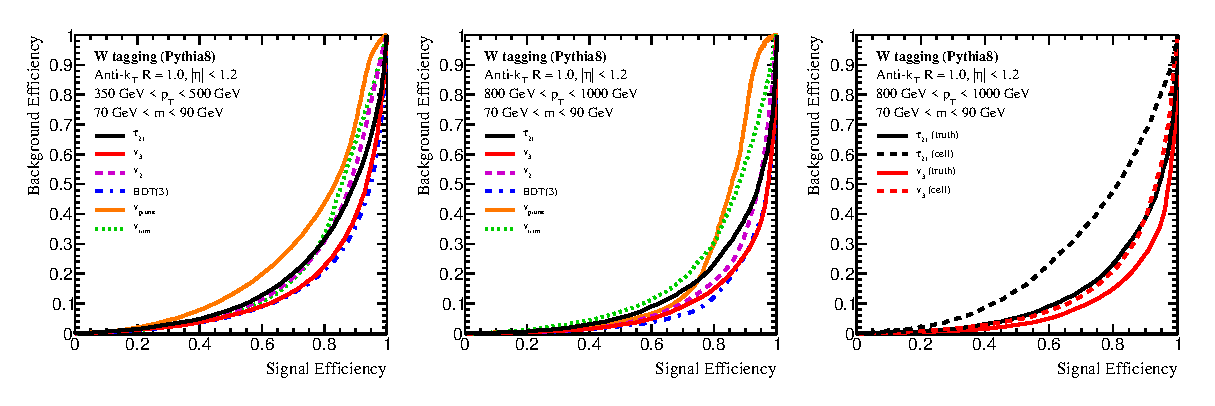
\includegraphics[width=2\columnwidth]{plots/W_ROCs_5.eps}
    \caption{The $W$ tagging ROC curves of the variabilities $v_2$, $v_3$, $v_{\rm trim}$, and $v_{\rm prun}$,
    the BDT combinations of three telescoping subjets variables $\{v_2, v_3, \theta_2\}$, and the two-prong tagger $\tau_{21}=\tau_{2}/\tau_{1}$, in the $(300~{\rm GeV}, 500~{\rm GeV})$ jet $p_T$ bin (left panel) and the $(800~{\rm GeV}, 1~{\rm TeV})$ bin (middle panel). Right panel: ROC curves of $v_3$ and $\tau_{21}$ in the $(800~{\rm GeV}, 1~{\rm TeV})$ jet $p_T$ bin. Solid curves correspond to the ones with the truth particle information, and the dashed curves are the ones using the pseudo-calorimeter cell particle information.}
\label{ROC_W}
\end{figure*}


The study is performed using samples generated from the Monte Carlo simulations of proton-proton collisions at $\sqrt{s}=13$ TeV using \textsc{Pythia8} \cite{Sjostrand:2007gs}. Particles are clustered into jets with \textsc{FastJet} 3~\cite{Cacciari:2011ma} using the anti-$k_T$ algorithm \cite{Cacciari:2008gp} with $R=1.0$ and are required to be central with a pseudorapidity $|\eta|<1.2$. We consider two kineamtic regimes, where the jet $p_T$ is between 350 GeV and 500 GeV or 800 GeV and 1 TeV. Signal $W$ boson and top quark jets are generated using decays of heavy Kaluza-Klein gravitons with an invariant mass at 1 or 2 TeV for the two $p_T$ bins in $gg\rightarrow G^*\rightarrow W^+W^-~{\rm or}~t\bar t\rightarrow {\rm hadrons}$. Background QCD jet are generated from the standard model dijet process. To study the impact of finite detector resolution, we compare the results with the particles clustered in pseudo-calorimeter $(\eta,\phi)$ cells of size $0.1\times 0.1$, with each cell momentum constructed with zero mass and direction from the primary vertex.  \textbf{\color{blue} SAM : Is there actually pileup overlaid?} Finally, in the case of telescoping subjets, jets are groomed using the trimming algorithm with $R_{\rm sub}=0.3$ and $f_{\rm cut}=0.05$ to remove the effects of pileup and a selection on the trimmed jet mass is made between 70 GeV and 90 GeV for $W$ tagging and between 160 GeV and 190 GeV for top tagging.

\begin{figure*}
    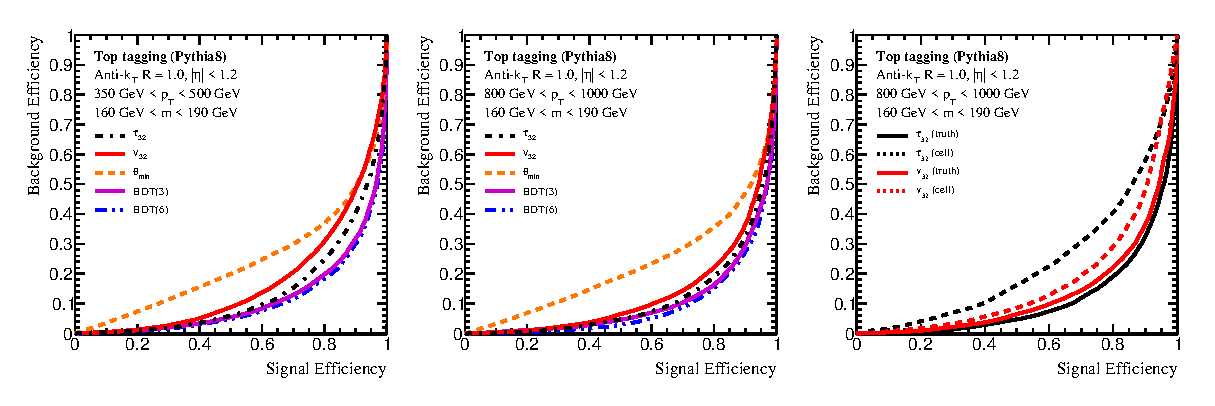
\includegraphics[width=2\columnwidth]{plots/Top_ROCs_1.eps}
    \caption{The top tagging ROC curves of the variability ratio $v_{32}$, the minimal angle among three subjets $\theta_{\rm min}$, the BDT combinations of three and six telescoping subjets variables $\{m_{W2},v_2,v_3\}$ and $\{\theta_2,\theta_{\rm min},m_{W2},v_2,v_3,v_{m_{W2}}\}$, and the three-prong tagger $\tau_{32}=\tau_{3}/\tau_{2}$, in the $(300~{\rm GeV}, 500~{\rm GeV})$ jet $p_T$ bin (left panel) and the $(800~{\rm GeV}, 1~{\rm TeV})$ bin (middle panel). Right panel: ROC curves of $v_{32}$ and $\tau_{32}$ in the $(800~{\rm GeV}, 1~{\rm TeV})$ jet $p_T$ bin. Solid curves correspond to the ones with the truth particle information, and the dashed curves are the ones using the pseudo-calorimeter cell particle information.}
\label{ROC_top}
\end{figure*}

To examine the complementarity of the information contained in the telescoping subjet variables, subsets of them are inputs for Boosted Decision Trees (BDTs) implemented in \textsc{TMVA} \cite{Hocker:2007ht}. For top tagging we also consider the ratio $v_{32}$ between $v_2$ and $v_3$,
\be
    v_{32}=\frac{v_3}{v_2}\;.
\ee
Shown in Figure~\ref{v32} are the distributions of $v_2$, $v_3$, and $v_{32}$ for top and QCD jets. We find that top jets have a broader $v_2$ distribution and a narrower $v_3$ distribution. The large variation of the jet mass when telescoping around the two subjet axes is caused by the transition of the $W$ from being partially reconstructed to fully reconstructed. There is not an intrinsic mass scale dictating the third hard emission for QCD jets. On the other hand, the three prongs inside top jets are quark-initiated subjets, whereas the subjets in QCD jets can have gluonic origins. Quark subjets are narrower than gluon subjets; therefore $v_3$ of top jets is statistically smaller. $v_{32}$ has almost the same performance as the BDT with input $\{v_2,v_3\}$, suggesting that $v_{32}$ may be the optimal way of combining the two variabilities. \textbf{\color{blue} SAM : The ideas being expressed here are jumbled and I cannot sort them out.  You need to try again since it comes off as just a laundry list of disjoint observations.}

An interesting feature of $v_{32}$ is that it cuts off naturally and sharply at 1, most clearly seen in QCD jets. Crucially, $v_{3} \leq v_{2}$. The two-prong structure in QCD jets implies that $v_{2}$ and $v_{3}$ collect almost the same information. The third energy flow axis can not be displaced far from the two axes determined at $N=2$. Hence, little new information is collected by constructing a third subjet and the distribution of $v_{32}$ for QCD jets peaks at 1. In the case where there is a third, semi-hard emission, the emission is captured by all telescoping subjets at $N=3$ and does not induce the observable variation and so $v_{3} < v_{2}$. In general, for larger $N$, more particles are and so the variability is expected to decrease ($v_{N+1}\leq v_{N}$).

The performances of the observables can be illustrated by receiver operating characteristic (ROC) curves, plotting the background efficiency as a function of the signal efficiency, where a lower curve indicates a better tagging performance. Shown in Figure~\ref{ROC_W} are the ROC curves of $v_2$, $v_3$, $v_{\rm trim}$, $v_{\rm prun}$, the BDT combinations of the telescoping subjet variables $\{v_2, v_3, \theta_2\}$, and the two-prong tagger $\tau_{21}=\tau_{2}/\tau_{1}$ in $W$ tagging. The left and middle panels correspond respectively to two jet $p_T$ regions of $(350~{\rm GeV}, 500~{\rm GeV})$ and $(800~{\rm GeV}, 1~{\rm TeV})$. Overall the tagging performance increases at higher $p_T$, demonstrating the general advantage of applying telescoping deconstruction to the boosted regime. We find excellent performance of $v_3$ and its qualitatively different feature compared to $\tau_{21}$. In the right panel we compare the tagging performance using truth particle information and pseudo-calorimeter clusters, which degrades information about structures smaller than the cell size. We find that $v_3$ is much more robust against this smearing, especially at high $p_T$. The $v_3$ observable utilizes the $W$ isolation and probes the rapid depletion of radiation around the $W$ at larger angles in the boosted regime. This is the manifestation of the fact that the $W$ carries zero color charge which affects the color structure of the subjets. The time dilation that occurs before $W$ hadronically decays can also create a huge difference from QCD jets in the jet formation process\textbf{\color{blue} SAM : I have no clue what you mean here or how you come to this conclusion based on this work.  It seems like vigorous hand waving.}. On the other hand, the fact that $v_3$ performs better than $v_2$ hints at the significance of a third hard emission in $W$ and QCD jets, and $v_3$ disentangles that effect in the quantification of the $W$ isolation. The physics picture of $v_{\rm trim}$ and $v_{\rm prun}$ is still under study.\textbf{\color{blue} SAM : I don't think this is an acceptable way to leave this paragraph.  It seems like disjoint observations but to just drop it as "and we don't understand this yet" is unsatisfying and makes the impression that we don't know whats going on.}

Shown in Figure \ref{ROC_top} are the ROC curves for top tagging performance including $v_{32}$, $\theta_{\rm min}$, the BDT combinations of telescoping subjets variables $\{v_2, v_3, m_{W2}\}$ and $\{\theta_2,\theta_{\rm min},m_{W2},v_2,v_3,v_{m_{W2}}\}$, and the three-prong tagger $\tau_{32}=\tau_{3}/\tau_{2}$. Again the left and middle panels correspond to the two kinematic regimes $p_T=(350~{\rm GeV}, 500~{\rm GeV})$ and $p_T=(800~{\rm GeV}, 1~{\rm TeV})$ and we note tagging performance increases at higher $p_T$. In the right panel the ROC curves plot both truth-particle and pseudo-calorimeter information. We find the excellent performance of $v_{32}$ and its robustness against smearing, especially at high $p_T$ where the performance of the more conventionally used $\tau_{32}$ observable degrades dramatically. This indicates the qualitatively different features of $v_{32}$ and a three-prong tagger\textbf{\color{blue} SAM : I don't understand this comment. Please clarify.}. We also find the usefulness of including $m_{W2}$ in the minimal BDT combination which significantly increases the tagging performance. It is clear that the intrinsic mass scale $M_W$ within the top jet is a unique feature distinguishing itself from the QCD background\textbf{\color{blue} SAM : But this is an obvious statement and we have attempted to eliminate it by making a mass cut *before* doing this study. This needs clarificiation.}. One may also start to see the $W$ isolation within the top jet in the boosted regime.

To conclude, we introduce a qualitatively new jet substructure calculus using variability to quantify the change of observables with respect to a sampling of the phase-space boundary in the observable definition. This method is general and can be used to analyze arbitrary classes of jet substructure observables and grooming procedures. In this context, when applied to $W$ and top tagging, we find excellent performance, especially in the case of telescoping subjet substructure, quantified via $v_3$ in $W$ tagging and $v_{32}$ in top tagging. Furthermore, their robustness is found to be significantly better than more widely used $N$-prong taggers such as $N$-subjetiness, via a comparison of the performance when reconstructed using truth particles as compared to a pseudo-calorimeter. 

The new physics messages we learn include the emergence of the isolation of $W$ jets at high $p_T$, which is a dominant feature over their two-prong structure. This is true for all other heavy, color-singlet Standard Model particles including the $Z$ and the Higgs boson. The top jet also has features beyond the three-prong structure which can be exploited to increase tagging performance. The telescoping subjets provides a systematic framework within which one can construct qualitatively new jet substructure observables. This paves the road toward complete and systematic jet studies using telescoping deconstruction \cite{Chien:2017decon} \textbf{\color{blue} SAM : I don't know what is trying to be said with this last paragraph, it seems like an afterthought.}.




\section{Acknowledgements}
Y.-T. Chien would like to thank the organizers of the BOOST2015 conference where telescoping jet substructure was first presented. Y.-T. Chien was supported by the US Department of Energy (DOE), Office of Science under Contract No. DE-AC52-06NA25396, the DOE Early Career Program and the LHC Theory Initiative Postdoctoral Fellowship under the National Science Foundation grant PHY-1419008. A. Emerman was supported by the National Science Foundation under Grant No. PHY-1707971. S.-C. Hsu and S. Meehan were supported by the DOE Office of Science, Office of High Energy Physics Early Career Research program under Award Number DE-SC0015971. Z. Montague was supported by the University of Washington's Ernest M. Henley \text{\&} Elaine D. Henley Endowed Fellowship.


\bibliography{TJet_ref}
\end{document}






















